\documentclass[../main/main.tex]{subfiles}


\begin{document}

\section{February 17th, 2020}
\subsection{More Laplace Transform}
Remember that the Laplace Transform for a function $f(t)$ is:
\[
	\mathcal{L}\{f(t)\} = \int^\infty_0 e^{-st}f(t)~dt = F(s)
.\] There is an associated inverse Laplace transform: \[
\mathcal{L}^{-1}\{F(s)\} = f(t)
.\] Which maps frequency space back to time space. If we avoid null functions, this inverse Laplace transform is unique, giving us tables of these pairs such as: 
\begin{table}[htpb]
	\centering
	\caption{Example of $\La$ and $\La^{-1}$ Pair Table}
	\label{tab:label}
	\begin{tabular}{c|c}
		$f(t)$ & $F(s)$\\\hline
		$t ^{m}e^{at}$ & $\frac{m!}{(s-a)^{m+1}},\quad s>a$\\
		$\sin(\omega t)$ & $\frac{\omega}{\omega^2+s^2},\quad s>0$\\
		\vdots& \vdots
	\end{tabular}
\end{table}
\begin{theorem} 
The Laplace transform is linear, i.e.: \[
	\La\{\alpha f(t) + \beta g(t)\} = \alpha\La\{f(t)\} + \beta\La\{g(t)\}
.\] 
\end{theorem}
\begin{remark}
	Proof in notes.
\end{remark}
\begin{example}
	 \[
		 \La\{t ^{3}e^{-t}+4\sin(8t)\} = \La\{t ^{3}e^{-t}\}+4\La\{\sin(8t)\} 
	.\] \[
	=\frac{3!}{(s-(-1))^{3+1}}+4\left( \frac{8}{8^2+s^2} \right) = \frac{6}{(s+1)^4}+\frac{32}{64+s^2}
.\] Note that the first term has condition $s>-1$ and the second has $s>0$, meaning that this domain is $s>0$.
\end{example}
\begin{remark}
	When there are multiple conditions, we take the intersection of the domains.
\end{remark}
\subsubsection{Limit Theorems}
\begin{theorem}[Limit Theorem]\index{limit theorems}
If $\La\{f(t)\}=F(s)\}$, we should find:  \[
		\lim\limits_{s \to \infty} F(s)=0
	.\] with the exception of some impulse functions.
\end{theorem}

\begin{example}
	We have $\La\{\cos(\omega t)\}= \frac{s}{s^2+\omega^2}$. Note that: \[
			\lim\limits_{s \to \infty} \left( \frac{s}{s^2+\omega^2} \right) =0
	.\] 
\end{example}
\begin{remark}
	This can be used as a check, as if you don't get $\lim\limits_{s \to \infty} F(s)=0$, and you aren't dealing with impulse function, then you did something wrong. 
\end{remark}
\begin{theorem}[Endpoint Theorem 1] \index{endpoint theorems}
	\[
		\lim\limits_{s \to \infty} (sF(s))=\underbrace{f(0^{+})}_{\lim\limits_{t \to 0^+} f(t)}
	.\]
\end{theorem}
\begin{example}
	Again consider $\La\{\cos(\omega t)\}$. We have: \[
		\lim\limits_{s \to \infty} s\left( \frac{s}{s^2+\omega^2} \right) =1
	.\] and \[
	\cos(\omega \times t) = 1
	.\] 
\end{example}

\begin{theorem}[Endpoint Theorem 2]
	 \[
		 \lim\limits_{s \to 0} (sF(s)) = \underbrace{f(\infty)}_{\lim\limits_{t \to \infty} f(t)}
	,\] provided it exists. 
\end{theorem}
\begin{remark}
	This allows us to the values of $f(t)$ without having to use the inverse Laplace transform.
\end{remark}
\begin{example}
	Suppose the Laplace transform of $f(t)$ is:  \[
		\La\{f(t)\} = \frac{1}{s\sqrt{s^2+1} }
	.\] We would like to find out what $f(0)$ and $f(\infty)$ are. Using the endpoint theorem, we have: \[
	f(0^{+}) = \lim\limits_{s \to \infty} s \frac{1}{s\sqrt{s^2+1} } = \lim\limits_{s \to \infty}  \frac{1}{\sqrt{s^2+1} } = 0
	.\] and \[
	f(\infty) \lim\limits_{s \to 0} s \frac{1}{s\sqrt{s^2+1} } = \lim\limits_{s \to 0} \frac{1}{\sqrt{s^2+1} }=1
	.\] 
\end{example}
\subsubsection{Existence of Laplace Transform of $f(t)$}
	Q: Can we take the integral of anything?\\
	A: No, as the Laplace transform is an improper integral, which must converge. 
	\begin{example}
		Note that  \[
			\La\{e^{t^2}\}=\int^\infty_0e^{-st}e^{t^2}~dt = \infty
		.\] Thus, $\La\{e^{t^2}\}$ does not have a Laplace transform.
	\end{example}
For a function to have a Laplace transform, it must be of exponential order.
\begin{definition}[Exponential Order] \index{exponential order}
	For a function $f(t)$ to be of \vocab{exponential order}, there must be a constant $\alpha$ for which: \[
		\lim\limits_{t \to \infty} e^{-\alpha t}f(t) = 0
	.\] 
\end{definition}
The function is allowed to go to infinity, just not too fast.
\subsubsection{Laplace Transforms for Derivatives}
Consider the Laplace transform of $f'(t)$ and use integration by parts with: \[
	\La\{f'(t)\} = \int^\infty_0 \underbrace{e^{-st}}_u \underbrace{f'(t)~dt}_{dv}
.\] \[
\underbrace{e^{-st}}_u\underbrace{f(t)}_v\bigg\rvert^\infty_0 - \int^\infty_0 \underbrace{f(t)}_v\underbrace{(-s e^{-st})~dt}_{du}  \]\[=\underbrace{e^{-\infty}}_0f(\infty) - \underbrace{e^{-0}}_1f(0^+) + s\int^\infty_0 f(t) e^{-st}dt = s\La \{f(t)\} -f(0^+)
.\] 
\begin{theorem}[Laplace Transform for Derivatives]
	\[
		\La \{f'(t)\} = s\La \{f(t)\} -f(0^{+}) 
	.\] 
	
\end{theorem}
\begin{example}
	Consider the second derivative: \[
		\La \{f''(t)\} = \La \{\frac{d}{dt}f'(t)\} =s\La \{f'(t)\} -f'(0^{+}) = s\left( s\La \{f(t)\} -f(0^+) \right) -f'(0^{+})
	.\] 
\end{example}
\begin{theorem}
	From the previous example: \[
		\La \{f''(t)\} = s^2\La \{f(t) \} -sf(0^+) -f'(0^+)
	.\] 
\end{theorem}
\begin{remark}
	This can be generalized, and as such we have: \[
		\La \{f'''(t)\} = s^{3}\La \{f(t)\} -s^2f(0^+)-sf'(0^+)-f''(0^+)	
	.\] Note that for each of the negative terms, the power of $s$ plus the order of the derivative of $f$ will equal the order of the derivative being computed minus 1, with the $s$ coefficient of $\La \{f(t)\} $ having the same power as the order.
\end{remark}
	Consider $ay''(t) + by'(t) + cy(t) = g(t)$  with initial conditions  $y(0) = y_0$, $y'(0) = y_0'$ and with $a,b,c$ being constant. Instead of solving by setting $g(t)=0 $, let us solve it using Laplace transform.\\
Let us begin by taking the Laplace transform of both sides: \[
	\La \{ay''(t) + by'(t) + cy(t)\} =\La \{g(t)\} 
.\] \[
\implies a\La \{y''(t)\} +b \La \{y'(t)\} +c\La \{y(t) \} = \La \{g(t)\} 
.\] \[
\implies a\large\left( s^2\La \{y(t)\} -sy(0^+)-y'(0^+) \large\right) +b\left( s\La \{y(t)\} -y(0^+) \right) +c\La \{y(t)\}  = \La \{g(t)\} 
.\] Thus we have: \[
\La \{y(t)\} = \frac{(as+b)y_0+ay_0'+\La \{g(t)\} }{as^2+bs+c}
.\] With this, we can get $y(t)$ by taking the inverse Laplace transform.

\begin{example}
	Consider: \[
		y''(t) + 2y'(t) + 3y(t) = t^3\quad y(0) = 0 \quad y'(0) = 1
	.\] With this we have: $a=1,b=2,c=3,y_0=0,y_0'=1$, and: \[
	\La \{g(t)\} =\La \{t ^{3} \} = \frac{3!}{s^{3+1}} = \frac{6}{s^{4}}
	.\] Thus without solving the ODE, we can say that: \[
	\La \{y(t) \} = \frac{(s+2)(0)+(1)(1)+\frac{6}{s^{4}}}{s^2+2s+3} = \frac{s^{4}+6}{s^{4}(s^2+2s+3)}
	.\] \[
	y(t) = \La ^{-1}\left\{ \frac{s^{4}+6}{s^{4}(s^2+2s+3)}\right\}
	.\] 
\end{example}
\subsubsection{Other Properties of Laplace Transforms}
\begin{theorem}[First Shifting Theorem]
	If $\La \{f(t)\} =F(s)$, then: \[
		\La \{e^{at}f(t)\} =F(s-a)
	.\] 
\end{theorem}
\begin{remark}
	The way to remember this, forget $e^{a t}$, and then whoever we get an $s$, replace by $s-a$.
\end{remark}
\begin{theorem}
	If $\La \{f(t)\} =F(s)$, then: \[
		\La \{tf(t)\} = - \frac{d}{ds}F(s)
	.\] \[
	\La \{t ^{m}f(t)\} = (-1)^{m} \frac{d^{m}}{ds^{m}}F(s)
	.\] 
	\end{theorem}
	\begin{remark}
		The way to do this, forget the $t$, then afterward take the derivative w.r.t. $s$ and negate it.
	\end{remark}
\begin{example}
	We have: \[
		\La \{e^{2t}\cos(4t)\} =\La \{\cos(4t)\} \bigg\rvert_{s\to s-2}
	.\] \[
=\frac{s}{s^2+4^2}\bigg\rvert_{s\to s-2} = \frac{s-2}{(s-2)^{2}+16}
	.\] 
\end{example}
\begin{example}
We have: \[
	\La \{t \cos(4t)\}  = \frac{d}{ds}\La \{\cos (4t)\} 
.\] 	\[
=-\frac{d}{ds}\left( \frac{s}{s^2+4^2} \right) =-\frac{d}{ds}\left( \frac{s}{s^2+16} \right) 
.\] \[
=-\left( \frac{\left( s^2+16 \right)-s(2s) }{\left( s^2+16 \right) ^2} \right) =\frac{s^2-16}{(s^2+16)^2}
.\] 
\end{example}
\begin{example}
We have: \[
\La \{t e^{-t}\sin(t)\} =\La \{t \sin(t)\} \bigg\rvert_{s\to s-(-1)}
\] 	\[
=-\frac{d}{ds}\La \{\sin(t)\} \bigg\rvert_{s\to s+1}= - \frac{d}{ds}\left( \frac{1}{s^2+1} \right) \bigg\rvert_{s\to s+1}
\] \[
=\frac{2s}{(s^2+1)^2}\bigg\vert_{s\to s+1}= \frac{2(s+1)}{\left( (s+1)^2+1 \right) ^2}= \frac{2s+2}{\left( s^2+2s+2 \right) ^2}
.\] 
\end{example}
\begin{remark}
	Knowing these two properties, then we can compute Laplace transforms of functions with factors of $t ^{m}e^{at}$.
\end{remark}
\subsubsection{Unit Step Function}
\begin{definition}[Unit Step Function]
	The \vocab{unit step function} $u_a(t)=u(t-a)$ is defined as: \[
		u_a(t) = \begin{cases}
			0,\quad t<a\\
			1,\quad t\ge a
		\end{cases}
	\] 
\end{definition}
\begin{figure}[h!]
	\centering
	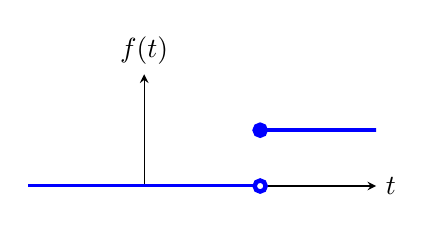
\begin{tikzpicture}
    \begin{axis}[width=6cm,height=3cm,domain=0:1,samples=501,ymin=0,ymax=1,xmin=-1,xmax=2,axis lines=center,
    xtick=\empty,ytick=\empty,
    xlabel={$t$},xlabel style={anchor=west},
    ylabel={$f(t)$},ylabel style={anchor=south}]
	\addplot[ultra thick,blue,mark=*,mark options={fill=white},samples at={-1.1,1}] {0};
\addplot[ultra thick,blue,mark=*,samples at={1,2.1}] {0.5};
    \end{axis}
\end{tikzpicture}
	\caption{ Example of a Unit Step Funciton}
	\label{fig:}
\end{figure}	
\noindent The Laplace transform for the unit step function is: \[
	\La \{u(t-a)\} =\int^\infty_0 u(t-a)e^{-st}~dt
\] \[
= \int^a_0(0)e^{-st}~dt + \int^\infty_a (1) e^{-st}~dt = - \frac{e^{-st}}{s}\bigg\rvert^\infty_a = \frac{e^{-as}}{s},\quad s>0
.\] 
\begin{remark}
	We can use this for calculating the Laplace transforms for piecewise functions.
\end{remark}
\begin{example}\label{piece}
	Consider the piecewise function\[
		f(t) = \begin{cases}
			0,\quad t<0\\
			1, \quad 0<t<2\\
			t,\quad2\le t\le 3\\
			e^{t},\quad3<t
		\end{cases}
	.\] We can express this as: \[
	1u(t) + (t-1) u(t-2)+(e^{t}-t)u(t-3)
	.\] 
\end{example}


Thus for any piecewise function, we can express it as: \[
	f(t) = \begin{cases}
		0,\quad t<0\\
		f_1(t), \quad 0<t<t_1\\
		f_2(t), \quad t_1<t < t_2 \\
		\vdots\\
		f_{m+1}(t),\quad t_m<t
	\end{cases}\]\[= f_1(t)u(t)+(f_2(t)-f_1(t))u(t-t_1) + (f_3(t)-f_2(t))u(t-t_2) +\ldots + (f_{m+1}(t)-f_{m}(t))u(t-t_m)
.\] 


\end{document}

